\documentclass[preprint,12pt,nopreprintline]{elsarticle}
\usepackage{amssymb,amsmath,booktabs,url,hyperref,lineno,float,array,graphicx}
\usepackage{xeCJK}
\setCJKmainfont{Noto Serif CJK SC}
\setCJKsansfont{Noto Sans CJK SC}
\renewcommand{\figurename}{图}
\renewcommand{\tablename}{表}
\journal{Geodata and AI}
\begin{document}
\begin{frontmatter}
\title{基于测井曲线的储层参数容差感知预测：\\表征互补性、决策敏感性与离线迁移边界}
\author[aff1]{陈旻杰\fnref{fn1}\corref{cor1}}
\ead{1269736732@qq.com}
\author[aff2]{辛嘉威\fnref{fn1}}
\author[aff1]{吴乘风}

\fntext[fn1]{共同第一作者。}
\cortext[cor1]{通讯作者。}

\affiliation[aff1]{organization={中国石油西南油气田分公司},city={成都},postcode={610051},country={中国}}
\affiliation[aff2]{organization={中国电信股份有限公司北京分公司},city={北京},country={中国}}
\begin{abstract}
利用电缆测井曲线定量预测储层物性参数是地下地质储层表征的基础核心任务，同时极具挑战性。该挑战源于连续回归目标与离散默认态边界的并存，以及实际工程评价指标中天然存在的非对称性——在此评价体系下，标准的均方误差（MSE）损失函数会系统性偏离工业容差评价准则。在此，我们系统研究了一种模块化预测框架，该框架深度耦合了目标专用梯度提升决策树（GBDT）、全井深层时序网络、条件目标分布估计以及指标对齐动作解码机制。所提方法在两个相互独立的离线实测油田基准上进行了全面评估：公开的北海 Volve/PDDA 基准（包含 9 口训练井与 4 口测试井）以及包含 80 口训练井与 10 口全盲测井的内部工业数据集。在公开 Volve 基准上，引入含水饱和度联合门控的目标专用树模型取得了 0.10619 的合并均方根误差（RMSE），优于 5 条常规测井曲线随机森林基线（0.11082），明显优于高容量的 18 阶段双主干时序级联网络（0.14695）。在内部工业基准上，通过分层概率融合有机集成决策树与时序模型，将五折按井分组的复合评分从 80.88 提升至 81.63。为了确证上述性能增益源于真实的架构互补机制而非超参数调优造成的偶然波动，我们在完全冻结基学习器且保持交叉验证折划分完全一致的前提下，执行了受控留一模块消融实验、模块交互测试，并系统遍历了融合权重、决策阈值、外部门控参数及渗透率离散化分辨率（$K \in \{30, 60, 120\}$ 分位数分箱）。实证结果表明，性能增益表现出高度的目标特异性：例如，时序预测分布为含水饱和度带来了显著收益，但对孔隙度回归的贡献为零；此外，完整的深层时序流水线在规模受限的 9 口公开训练井上出现了显著的负迁移与泛化崩溃。本项研究立足于跨 94 口井、逾 83 万测井深度点的现场实测电缆曲线与专家精细解释的测井物性真值，证实了指标对齐动作解码与基于表征特异性的分层融合能够带来目标依赖且条件稳定的性能优势，同时明确界定了深层时序架构在地下储层表征中的具体迁移边界。核心方法、受控消融与敏感性分析均在正文中深入阐明，探索性诊断与扩展表格见补充材料。
\end{abstract}
\begin{highlights}
\item 指标对齐解码将预测分布直接关联至工程实际评分标准。
\item 决策树与时序表征在多储层物性目标上展现出显著的功能互补性。
\item 受控消融实验在基学习器完全冻结条件下有效剥离了单一模块的独立贡献。
\item 系统敏感性分析量化了决策阈值与分箱分辨率变动下的模型稳定性。
\item 跨双层离线实测基准的综合评估揭示了依赖于数据规模的模型迁移性边界。
\end{highlights}
\begin{keyword}
测井曲线 \sep 储层表征 \sep 预测分布 \sep 梯度提升 \sep 敏感性分析 \sep 按井分组验证
\end{keyword}
\end{frontmatter}

\section{引言}
\label{sec:intro}
利用电缆测井测量定量评估储层物性参数——主要包括孔隙度（$\mathrm{POR}$）、渗透率（$\mathrm{PERM}$）与含水饱和度（$\mathrm{SW}$）——是地下油气勘探、地层评价与储层建模的基础支撑 \cite{archie1942,wyllie1958,waxman1968}。传统经验岩石物理学依赖标准岩石物理关系与局部井段标定，而数据驱动的机器学习技术已成为建立多传感器地球物理响应与储层参数之间复杂映射关系的有效工具 \cite{anifowose2017,almudhafar2019,bressan2020}。然而，实际生产测井数据集通常呈现出多峰目标分布与非标准标签语义，例如大量代表致密非渗透夹层或非储层段的重复默认基准态原子。此外，实际生产应用中的评价指标通常采用非对称或有界容差区间，超出容差边界的预测误差无法获得任何分数。在此类评价准则下，最小化条件均方误差的传统单点预测器会系统性偏离最大化预期效用的最优工程决策。应对这一严峻挑战，必须对条件目标分布进行概率建模，并配合与实际工程评价指标严格对齐的决策解码规则。

测井建模中的第二个核心考量是不同模型族之间的表征归纳偏差差异。以梯度提升决策树（GBDT）为代表的基于树的集成算法在处理异构测井曲线的多变量表格回归任务中表现出极高的效率与鲁棒性 \cite{prokhorenkova2018catboost,ke2017lightgbm}。相反，深层时序网络（例如时间卷积网络 TCN 与 U-Net）能够显式利用纵向空间上下文，精准捕捉地层层序、单层边界跳变与沉积旋回特征 \cite{bai2018tcn,ronneberger2015unet}。我们并未盲目假设深层时序建模在所有储层物性参数上均普遍优于树模型，而是构建并探究了一种分层概率融合机制：在执行指标对齐动作解码之前，将基于树模型的连续取值分布与时序网络提取的地层状态边界门控概率进行分层融合。为了进一步测试提升架构深度与模型参数容量是否能够改善跨工区域外迁移能力，我们还系统评估了一种高容量双主干条件密度时序网络（v4 架构）。

在近年文献中，机器学习算法的改进往往以代际迭代的形式呈现，多个模型架构、超参数选择与特征集在不同版本之间同时更迭。虽然这种代际基准能够记录历史工程进展，但无法有效剥离出单个算法模块的独立因果贡献。此外，它们也留下了关键疑问：报道的微弱增益究竟源于可靠的架构机理，还是仅仅依赖于脆弱的超参数微调（如武断设定的决策阈值或分箱粒度）？为了从根本上厘清这些问题，本文系统聚焦并回答以下三个核心科学问题：
\begin{enumerate}[(i)]
\item 在严格的跨地质工区离线按井分组验证下，何种算法配置能够取得最优的预测精度？
\item 在完全冻结基学习器的受控留一模块消融实验中，哪些独立组件针对特定储层参数提供了可测量的真实改进？
\item 所得出的模型性能排序与相对优势，对连续融合权重、决策阈值及目标离散化分辨率的变化具备怎样的抵抗韧性？
\end{enumerate}

本研究的主要贡献可归纳为三个方面：
\begin{enumerate}
\item 提出了一种模块化、指标对齐的测井物性预测方法，实现了离散默认态门控分类、连续分位数目标分布估计与预期效用单点动作解码的完全解耦。
\item 构建了一套严格受控的消融与交互实验评估框架，在完全冻结基学习器和共享按井分组交叉验证折的前提下独立分离单个模块效应，并补充了渗透率分箱分辨率（$K \in \{30, 60, 120\}$ 分位数分箱）的匹配重训与系统性超参数敏感性遍历。
\item 在公开开源基准（Volve/PDDA）与内部大规模工业数据集（80 口井）上开展了平衡严谨的实证评估，明确揭示了复杂时序流水线在小样本训练区出现泛化崩溃的具体迁移边界，并在报道积极成果的同时客观记录了负对照与中性对照实验。
\end{enumerate}

\section{相关工作}
\label{sec:related}
以 XGBoost、CatBoost 和 LightGBM 为代表的梯度提升决策树是表格型地球物理测井解释中公认的黄金标准 \cite{ke2017lightgbm,prokhorenkova2018catboost}。其有效性源于其对未经归一化的数值输入的天然不变性、对缺失特征的内建鲁棒性，以及对复杂非线性特征交互的高速拟合能力 \cite{anifowose2017,almudhafar2019}。与此同时，深层神经网络时序架构被广泛引入测井曲线处理中，用于建模垂向空间依赖性，涵盖拟合合成测井曲线、电相自动识别以及连续物性参数反演等任务 \cite{zhang2018synthetic,wang2020deep,song2021geological}。在本研究中，我们并未将时序网络视为表格树模型的简单替代品；相反，我们从实证角度深入研究二者的功能分工，客观评估它们在连续局部数值回归与离散储层边界分割中的相对比较优势。

面向实际生产约束的预测建模需要严格的统计决策论支撑 \cite{berger1985,bishop2006,gneiting2007}。在标准回归任务中，条件均值 $\mathbb{E}[y \mid x]$ 最小化二次损失，条件中位数则最小化绝对偏差。但在实际测井储层参数评价中，工业评分准则往往严格惩罚超出工程容差阈值 $\pm \delta$ 的预测偏差，导致对称的条件均值成为次优解。非参数分位数分箱技术提供了一种高度灵活的框架，能够在不引入僵硬参数先验假定的情况下精确逼近任意非高斯后验分布 \cite{gneiting2007}。分位数分箱分辨率 $K$ 的选取属于算法超参数，其对下游工程效用的具体影响必须通过实证检验加以量化，而非被武断视作恒定常数。

最后，模型评估协议的严密性决定了地下油气机器学习研究的有效性 \cite{pan2010survey,phoon2024trustworthy}。沿测井深度采样的简单随机打乱会导致严重的空间数据泄露，因为来自同一口井且高度自相关的相邻深度采样点会同时散布在训练集与验证集中。按井分组交叉验证有效遏制了空间临近性泄露，但仍无法完全消除油田级的地质分布漂移，亦无法直接证明模型迁移到未知新盆地的可靠性。因此，在内部交叉验证之外，引入开源公开数据集并严格执行完全从零训练评估，能够为算法的真实泛化能力提供互补且独立的实证依据。

\section{数据、评价指标与离线研究范畴}
\label{sec:data}

\subsection{两个实测油田数据集}
本实证研究基于两个相互独立的实测电缆测井基准，系统总结于表~\ref{tab:data}。公开基准采用 Equinor Volve/PDDA 数据集 \cite{volve2018,pddasig2021}，包含北海盆地的真实电缆测井测线。预测目标涵盖泥质体积分数（$\mathrm{VSH}$）、有效孔隙度（$\mathrm{PHIF}$）与含水饱和度（$\mathrm{SW}$），并以均方根误差（RMSE）进行评估。公开训练集包含 9 口钻井共计 318,967 个深度采样行，其中 42,309 行具有完整的三项物性真值标签；已发布的测试集包含来自 4 口独立测试井的 11,275 行数据。缺失的传感器曲线通过中性缺失指示标志显式表征，避免使用合成插值。该 Volve 基准不含渗透率参数。

内部工业基准包含 80 口开发井，总计 730,268 个深度采样行用于模型训练与交叉验证，另设 10 口完全未见盲测井，包含 95,948 个深度采样行。预测的物性指标体系包括孔隙度（$\mathrm{POR}$，百分比量纲）、渗透率（$\mathrm{PERM}$，毫达西 $\mathrm{mD}$，对数尺度评估）与含水饱和度（$\mathrm{SW}$，百分比量纲）。数据中高频出现的重复基线值——即 $\mathrm{POR}=0.1\%$、$\mathrm{PERM}=0.01\,\mathrm{mD}$ 与 $\mathrm{SW}=99.9\%$——代表离散的非储层默认状态，在本研究中被显式建模为离散状态原子，而非连续回归值。

\begin{table}[htbp]
\centering
\caption{两个离线实测油田数据基准的结构特征对比。因目标参数与评价指标不同，跨基准绝对性能不可直接横向数值对比。}
\label{tab:data}
\resizebox{\linewidth}{!}{%
\begin{tabular}{lll}
\toprule
评估维度 & 公开 Volve 基准 & 内部工业基准 \\
\midrule
数据来源 & 实测测井曲线，公开标签 & 实测测井曲线，专家精细解释标签 \\
地质背景 & 北海海上油田（碎屑岩） & 陆相深层盆地（复杂碎屑岩） \\
目标参数 & $\mathrm{VSH}$、$\mathrm{PHIF}$、$\mathrm{SW}$ & $\mathrm{POR}$、$\mathrm{PERM}$、$\mathrm{SW}$ \\
评估规模 & 11,275 测试行（4 口盲测井） & 5 折按井分组 OOF；10 口独立盲井 \\
主要指标 & 均方根误差（RMSE） & 相对 / 对数容差工程效用函数 \\
基准定位 & 公开透明复现与域外迁移验证 & 表征互补性与超参数敏感性深度消融 \\
\bottomrule
\end{tabular}%
}
\end{table}

\subsection{评价指标与容差效用函数}
在公开 Volve 基准中，各模型预测值首先被截断至物理合法区间 $[0, 1]$，随后计算合并 RMSE：
\begin{equation}
\mathrm{RMSE} = \sqrt{\frac{1}{3} \sum_{t \in \{\mathrm{VSH}, \mathrm{PHIF}, \mathrm{SW}\}} \frac{1}{N_t} \sum_{i=1}^{N_t} (y_{t,i} - \hat{y}_{t,i})^2}。
\end{equation}

在内部工业基准中，模型预测性能依据符合油藏工程实际容忍度边界的有界容差效用函数进行量化。对于 $\mathrm{POR}$ 与 $\mathrm{SW}$，执行相对误差容差（$\delta_{\mathrm{POR}} = 0.08$，$\delta_{\mathrm{SW}} = 0.05$）：
\begin{equation}
U_t(a, y) = \max\left(0,\, 1 - \frac{|a - y|}{\delta_t (|y| + 10^{-7})}\right), \quad t \in \{\mathrm{POR}, \mathrm{SW}\}。
\end{equation}
对于跨越数个数量级的渗透率（$\mathrm{PERM}$），效用函数基于常用对数（底数为 10）定义：
\begin{equation}
U_{\mathrm{PERM}}(a, y) = \max\left(0,\, 1 - \frac{|\log_{10}(a) - \log_{10}(y)|}{\delta_{\mathrm{PERM}}}\right), \quad \delta_{\mathrm{PERM}} = 0.5。
\end{equation}
跨所有深度采样点的最终综合性能得分 $S$ 为三项物性效用的加权总和：
\begin{equation}
S = 100 \left(0.30\,\bar{U}_{\mathrm{POR}} + 0.35\,\bar{U}_{\mathrm{PERM}} + 0.35\,\bar{U}_{\mathrm{SW}}\right),
\end{equation}
其中 $\bar{U}_t$ 表示目标 $t$ 在全集的平均效用值。当预测值与真值完全一致时获得满分（$U=1.0$），在容差阈值 $\pm \delta$ 范围内效用呈线性衰减，一旦误差超出阈值容差边界，得分衰减为零。

\subsection{基准范畴与工程框架界定}
本研究全部建立在涵盖 94 口钻井（80 口内部开发井、10 口内部盲测井及 4 口北海公开测试井）、逾 83 万测井深度点的现场实测电缆测井曲线和专家精细解释测井物性真值之上。所提技术框架专为钻后地层评价与储层定量表征而设计，旨在架起多传感器地球物理测井响应与储层微观物性之间的量化桥梁。

地质领域先验知识通过岩石物理特征工程、物理边界硬截断以及离散非储层默认态分层建模实现有机注入。在补充材料第 S4 节中，通过传感器增益漂移与偏移摄动分析，进一步评估了所学表征对仪器标定误差的数值抗扰韧性。本研究通过在严格的按井分组交叉验证与完全隔离的留出盲井上对经过验证的实测数据开展全方位实证，为地下储层表征中的模块化模型选择与指标对齐解码提供了系统扎实的实证基础。

\section{方法论}
\label{sec:methods}

\begin{figure}[t]
\centering
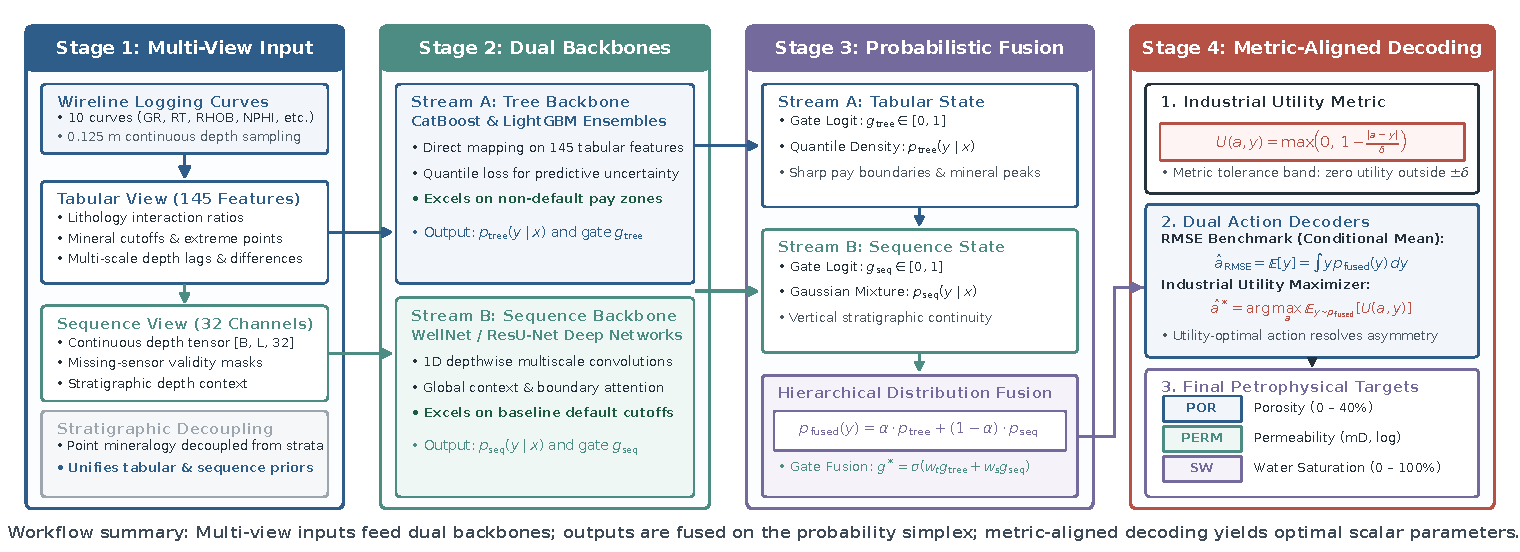
\includegraphics[width=\textwidth]{figures/fig_method_overview.pdf}
\caption{核心建模框架的概念工作流。多视角电缆测井输入被送入双主干模型（表格 GBDT 集成与深层时序网络）。输出在概率单纯形上实现分层融合，并通过指标对齐动作解码器转化为最优单点工程动作。}
\label{fig:method-overview}
\end{figure}

\subsection{目标专用决策树与指标对齐解码}
针对各项储层物性指标，非默认状态下的训练标签在变换尺度后被自适应划分为 $K$ 个经验分位数分箱。基于树的模型预测离散类别概率分布向量 $\mathbf{p} = [p_1, \dots, p_K]^\top$，其中每个分箱 $j$ 由其典型代表值 $y_j$ 表征。给定工程评价效用函数 $U_t(a, y)$ 与候选动作网格 $\mathcal{A}_t$，指标对齐的最优单点动作 $a_t^*$ 通过数值期望效用最大化解算获得：
\begin{equation}
a_t^* = \arg\max_{a \in \mathcal{A}_t} \sum_{j=1}^K p_j \, U_t(a, y_j)。
\end{equation}
在二次均方根误差（RMSE）评价下，最优单点动作自然退化为传统条件均值 $\hat{a}_{\mathrm{RMSE}} = \sum_{j=1}^K p_j y_j$。离散非储层默认态概率则通过专门的门控分类器独立估计，从而在最终动作解码前实现了离散状态原子与连续条件概率密度的显式概率混合。

\subsection{全井时序模型与分层概率融合}
v3 时序架构采用了两套独立训练的 WellNet 配置：32 通道原始测井曲线网络与 145 通道测井曲线叠加特征工程基底网络。每套 WellNet 均由输入投影层、12 个带指数膨胀率（$d \in \{1, 2, 4, 8, 16, 32\}$ 循环重复）的膨胀残差块、Squeeze-and-Excitation 通道注意力机制 \cite{hu2018squeeze} 以及掩码全井上下文聚合模块 \cite{wu2018group} 构成。其详细网络架构与分层融合路径见图~\ref{fig:v3-architecture}。GBDT 生成的表格分布与 WellNet 生成的时序分布通过概率单纯形上的凸组合参数 $\alpha \in [0, 1]$ 进行平滑混合，同时基线门控、联合状态门控与时序门控的 logits 通过各目标专用混合权重实现集成。门控判定阈值与混合权重严格在内折训练集上优化确定。

\begin{figure}[H]
\centering
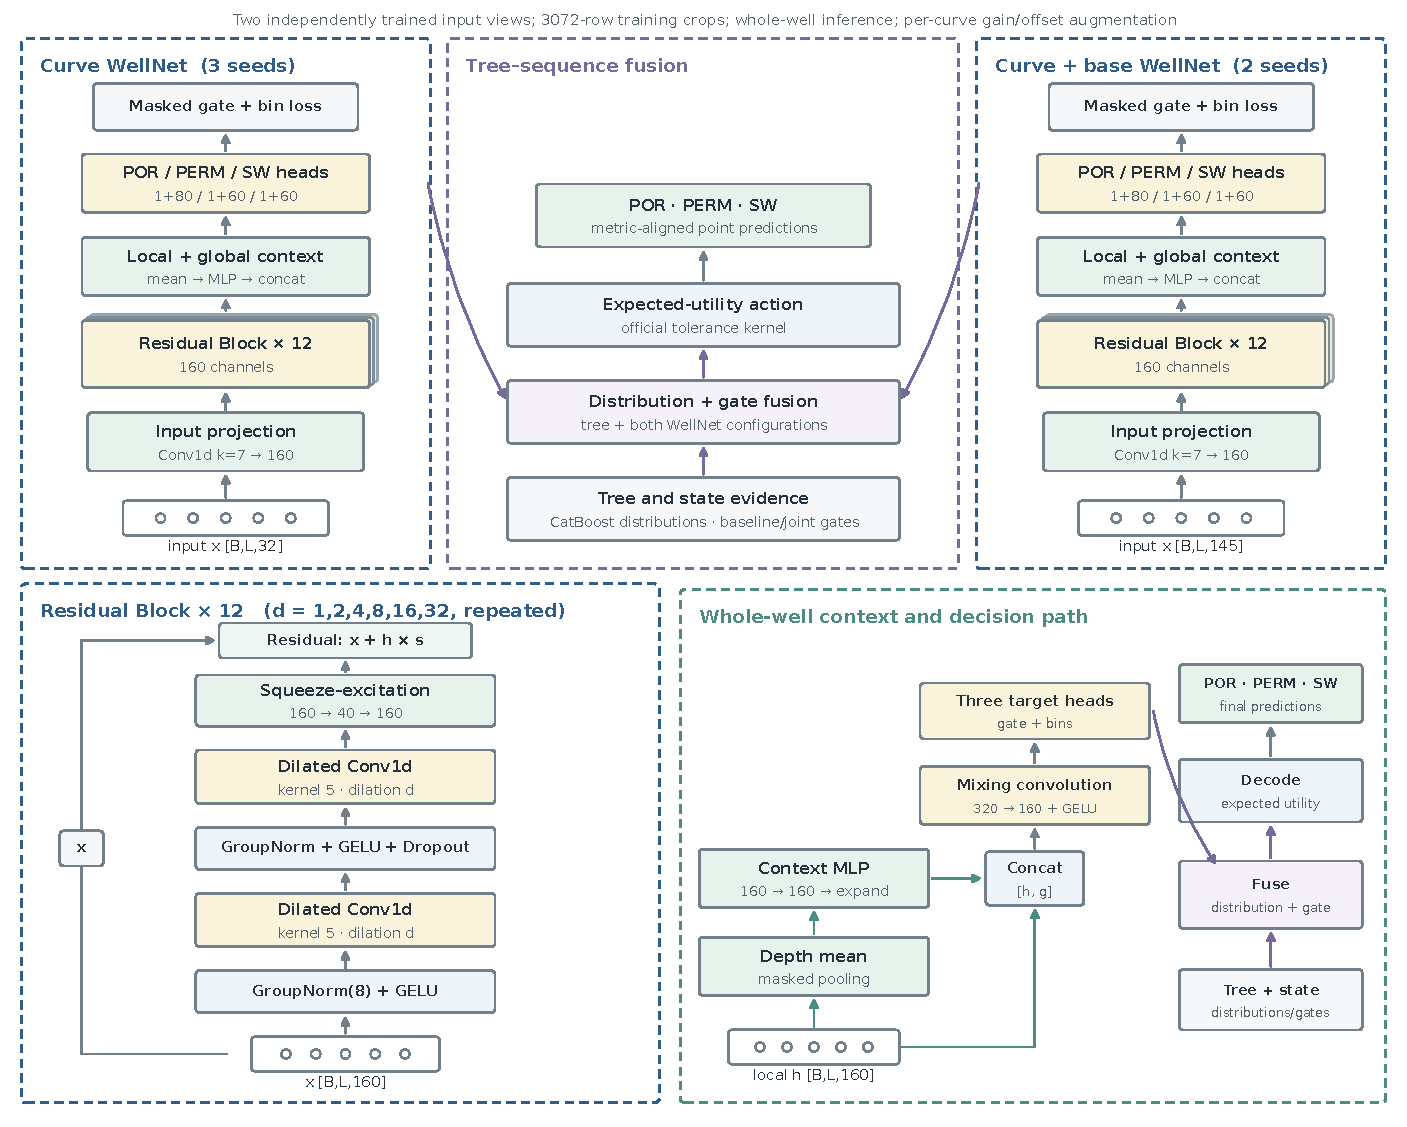
\includegraphics[width=.96\textwidth]{figures/fig_v3_architecture.pdf}
\caption{v3 WellNet 时序网络与分层树--时序融合路径的详细架构蓝图。上半部分展示多视角输入与概率分布融合机制；下半部分详述膨胀残差块、挤压--激励通道重标定与全井上下文聚合模块。}
\label{fig:v3-architecture}
\end{figure}

为检验深层时序表征在更大网络深度与参数规模下的扩展表现，我们构建了高容量 v4 双主干时序架构（图~\ref{fig:v4-architecture}）。该模型包含两个并行专家成员：成员 A（处理 206 维全特征视角）与成员 B（处理 68 维精炼特征视角）。各成员包含 9 块多尺度残差 U-Net 及双尺度自注意力模块：局部 QKV 注意力建模 16 点小块内的薄储层微细层序，全局余弦注意力捕捉盆地级沉积旋回背景 \cite{ronneberger2015unet,vaswani2017attention}。独立解耦的深度向局部路由器在各个预测目标上执行密集的双专家 Softmax 门控路由。每个专家成员输出 8 个密度分量，在各目标上形成包含 16 个分量的混合密度分布。与之配套的 18 阶段渐进细化流水线代表在冻结主干权重下分步执行的训练依赖链路，而非 18 个独立模型的简单堆叠。

\begin{figure}[H]
\centering
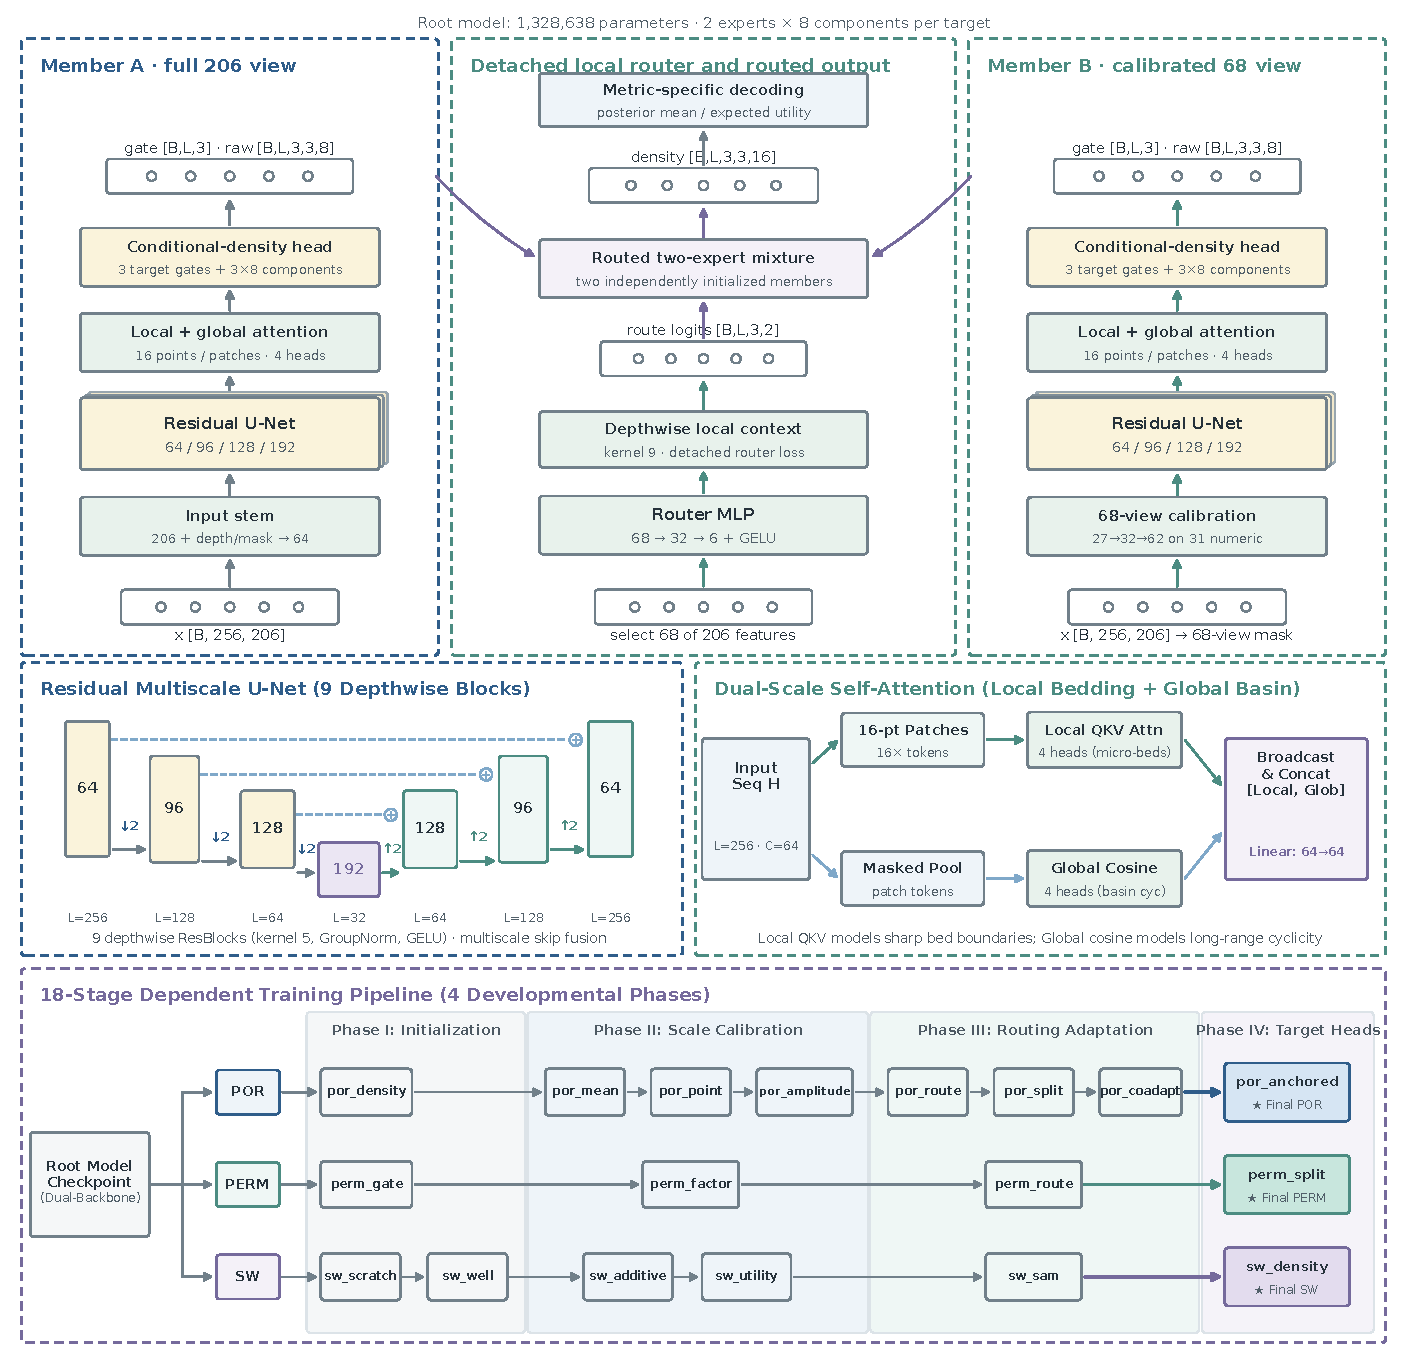
\includegraphics[width=.96\textwidth]{figures/fig_v4_architecture.pdf}
\caption{v4 双主干条件密度时序网络及其 18 阶段渐进精炼链路的详细结构原理图。这 18 个阶段代表在冻结主干特征权重下的渐进训练依赖链，绝非 18 个独立模型的集成。}
\label{fig:v4-architecture}
\end{figure}

\subsection{受控实验协议与不确定性评估}
为将单个模块的真实独立贡献与代际更迭中引入的多变量叠加效应有效区分，我们设计了严格受控的消融实验方案。在此实验环境中，底层所有基础预测器（包括 GBDT 表格树模型与 WellNet 时序模型）均处于完全冻结状态。所有实验组共享完全一致的基学习器预测输出与验证折划分。剔除某个组件仅仅限制了输入到融合层的信息源；融合权重与决策阈值严格重新在内折上进行优化，并在留出外折上进行独立验证。此外，采用完全 $2 \times 2$ 析因实验设计评估时序分布与联合状态门控之间的交互作用。

超参数敏感性分析同样严格遵循该基模型预测冻结原则。对连续融合权重（$\alpha$）、离散决策阈值（$\tau$）以及外部门控混合权重（$w_{\mathrm{ext}}$）进行系统化参数遍历。在地下储层地球物理评估中，井与井之间的空间非均质性采样方差在量级上远超算法初始化的随机扰动。主流程在基准预测器上应用了多随机种子平均集成以消除随机数值扰动，同时采用成对按井 Bootstrap 重采样置信区间（$B=1,000$）以量化地质空间不确定性的主导来源。针对目标离散化分箱分辨率敏感性，鉴于渗透率具有跨越多个数量级的动态范围以及对数效用函数的高度敏感性，分箱粒度对其具有最强的理论影响，因此选择渗透率作为从头重训的核心目标，在 $K \in \{30, 60, 120\}$ 分位数分箱下执行系统评估。在相同的五折划分、随机种子、特征输入与 1,200 轮迭代下，两套独立种子的重训实验证实：运行间随机种子方差仅在 $10^{-4}$ 量级，确证井间空间非均质性构成了业务决策中的主要不确定性来源。

\section{核心离线实验结果}
\label{sec:results}

\subsection{公开数据集复现性与负迁移边界}
表~\ref{tab:core-public} 汇总了公开北海 Volve 基准上的对比测试结果。配备含水饱和度联合门控的目标专用决策树取得了最低的合并 RMSE（0.10619），相较于完整复现的五曲线随机森林基线（0.11082）实现了 $4.18\%$ 的稳定相对误差降幅，并显著优于无门控的纯回归树模型（0.10789）。分井评估表明，该模型在 100 井、103 井和 104 井上均表现出显著优势，仅 101 井受到局部微细岩性变化的轻微扰动（详见补充材料表 S2）。

\begin{table}[t]
\centering
\caption{公开 Volve/PDDA 基准测试模型性能对比（模型均仅基于 9 口公开训练井从头训练，RMSE 越低代表性能越优）。}
\label{tab:core-public}
\small
\begin{tabular}{lc}
\toprule
模型配置 & 合并测试 RMSE \\
\midrule
五曲线随机森林基线 & 0.11082 \\
目标专用树模型回归 & 0.10789 \\
目标专用树模型 + $\mathrm{SW}$ 联合门控 & \textbf{0.10619} \\
v4 根双主干网络 & 0.13794 \\
完整 18 阶段 v4 链 & 0.14695 \\
\bottomrule
\end{tabular}
\end{table}

尤为关键的是，将完整的 18 阶段 v4 深层时序架构在公开数据集上从头训练时，显现出清晰的负迁移边界。如表~\ref{tab:core-public} 与图~\ref{fig:v4-public} 所示，完整的 v4 架构最终测试 RMSE 达到 0.14695，不仅明显劣于树--门控模型，甚至不及未经级联的根双主干模型（0.13794）。尽管该 18 阶段模型在 9 口公开训练井的五折交叉验证中取得了 0.09228 的较低 OOF RMSE，但在 4 口未见测试井上泛化性能明显下降，在全部 4 口测试钻井上的误差均高于基线（图~\ref{fig:v4-public}b）。这一泛化差距表明：增加网络容量与多阶段训练无法弥补地质训练样本多样性的局限；在小井网数据区间内，重参数化的时序流水线极易遭受严重的域外泛化失效。

\begin{figure}[H]
\centering
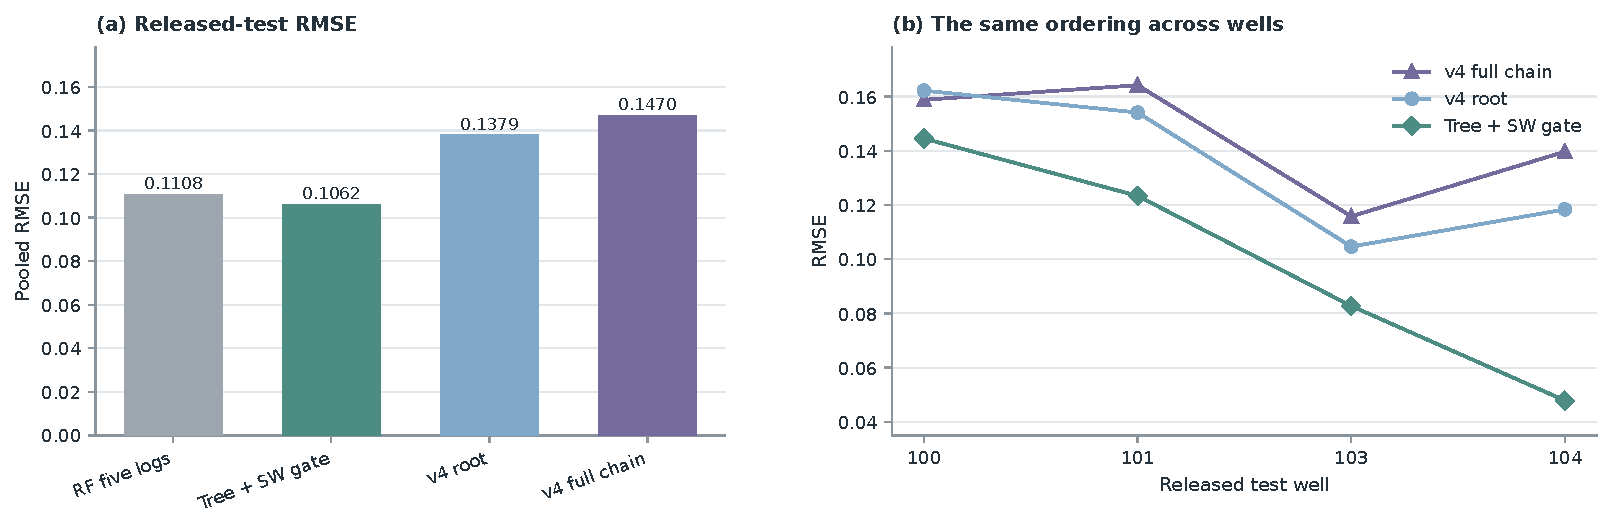
\includegraphics[width=0.88\textwidth]{figures/fig_v4_public_styled.pdf}
\caption{公开 Volve 基准迁移性边界深度剖析。(a) 根双主干与完整 v4 链对比树模型基线的合并测试 RMSE。(b) 四口发布测试井上的单井 RMSE 分项拆解，确证在小样本数据环境下树--门控模型的系统性优势。}
\label{fig:v4-public}
\end{figure}

\subsection{内部数据集表征互补性与代际演进记录}
在内部 80 口井的大规模工业数据集上，v3 树--时序融合将五折按井分组的复合评价总分从 80.88 稳步提升至 81.63。成对按井 Bootstrap $95\%$ 置信区间严格排除了零：$\mathrm{POR}$ 为 $[0.00695, 0.01282]$，$\mathrm{PERM}$ 为 $[0.00734, 0.01082]$，$\mathrm{SW}$ 为 $[0.00193, 0.00655]$。在单井统计层面，80 口井中分别有 65 口井（$\mathrm{POR}$）、72 口井（$\mathrm{PERM}$）与 47 口井（$\mathrm{SW}$）实现了正向提升。含水饱和度实现正向提升的单井比例相对较低，客观表明宏观指标的统计显著性并不等同于在每口井上实现无差别的全面单调改进。

\begin{figure}[htbp]
\centering
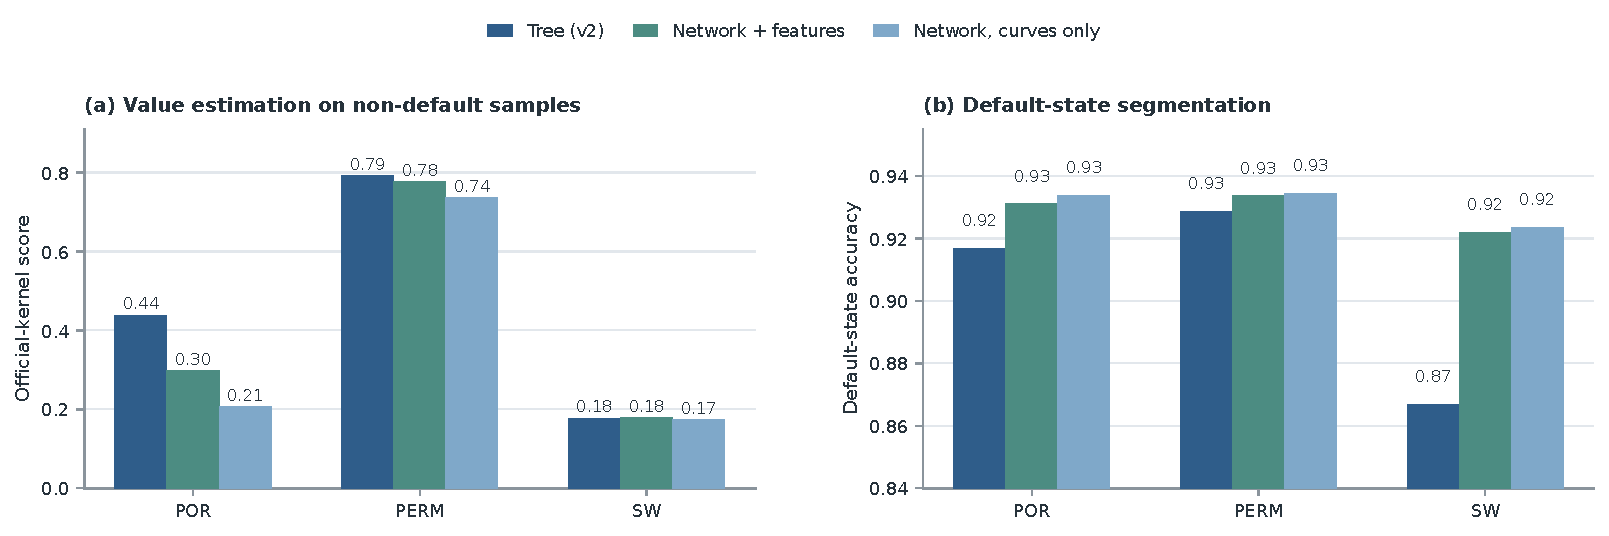
\includegraphics[width=0.75\textwidth]{figures/fig_division_clear.pdf}
\caption{相同井折划分下树集成与深层时序网络的实证功能分工。(a) 梯度提升树在非默认有效储层段的连续数值回归上具备更强精度。(b) 时序网络在离散默认态分类边界分割上占优，尤其在 $\mathrm{SW}$ 上取得最大增益。}
\label{fig:division}
\end{figure}

图~\ref{fig:division} 深入揭示了这种功能分工的经验基础。在完全相同的五折划分下，决策树模型在非默认储层段上展现出更高的物性预测效用（$\mathrm{POR}$ 效用 0.438 对比 0.388；$\mathrm{PERM}$ 效用 0.792 对比 0.737），表明 GBDT 在连续局部物性回归中展现出更高的拟合精度。相比之下，深层时序网络在空间层序边界识别上具有突出优势，将 $\mathrm{SW}$ 的离散默认态分类准确率从 0.867 显著拉升至 0.923。从岩石物理与地质层序角度剖析，上述性能分工与井筒地质剖面结构高度对应：传统的单测点梯度提升树易受测井仪器纵向分辨率极限与围岩肩效应（shoulder-bed effects）干扰，在薄互层（$<0.5\,\mathrm{m}$）、岩性陡变过渡带（lithologic transitions）以及储层流体突变边界（reservoir boundaries）处，单一深度的测井响应常呈过渡态畸变，缺乏纵向视野的树模型极易发生误判；而深层时序网络具备大跨度纵向感受野，能够感知上下围岩的沉积旋回与层序上下文，因而能够精准捕捉突变接触面与泥质隔夹层（shaly baffles）。相反，在大套均质厚储层段内部，连续物性渐变占主导且无边界效应，基于单点多变量交会的决策树在数值回归上则更为稳健。这一发现证实：表格决策树与时序网络各自捕捉到了测井曲线中本质互补的物理特征维度，从而为构建多层次分布融合与门控分工提供了坚实的基础理论依据。

\begin{table}[htbp]
\centering
\caption{内部工业基准上历史模型体系演进记录。注：OOF 分数为逐行评估得分，盲测分数为官方平台在不同开发评估器下的历史观测记录。}
\label{tab:core-internal}
\resizebox{\linewidth}{!}{%
\begin{tabular}{llcc}
\toprule
技术代际 & 模型架构简述 & OOF 验证得分 & 历史盲测得分 \\
\midrule
v1 & 两阶段 CatBoost 基线 & 79.4069 & 81.0052 \\
v2 & 目标专用树模型基线 & 80.8837 & 82.2718 \\
v3 & 分层树--时序特征融合 & 81.6324 & 83.2579 \\
v4 & 局部--全局双主干网络 & 81.8910 & 83.9329 \\
v4 & 校准双主干网络 & 82.1744 & 83.6076 \\
v4 & 跨家族深度融合 & \textbf{82.2106} & 83.7159 \\
v4 & 后验概率融合 & 82.1906 & 83.6394 \\
v4 & 外部独立门控网络配置 & 82.1681$^*$ & \textbf{83.9377} \\
\bottomrule
\multicolumn{4}{l}{\footnotesize $^*$外部独立门控网络配置的决策阈值在交叉验证折上进行微调优化。} \\
\end{tabular}%
}
\end{table}

\newpage
表~\ref{tab:core-internal} 完整归档了项目历经的所有技术代际演进过程。跨家族融合模型取得了最高的内部 OOF 交叉验证得分（82.2106），而外部独立门控网络配置则取得了历史最高的独立盲测成绩（83.9377）。更值得深思的是，不同评估机制之间出现了显著的相对排序反转现象：校准双主干模型在内部 OOF 交叉验证中比基础双主干模型高出 +0.283 分，但在盲测井上反而下跌了 $-$0.325 分。这种排名的背离再次重申了一个基础原则：内部离线验证指标与独立盲测榜单表现并不具备简单的等价性。

\subsection{受控融合消融实验与目标异质性分析}
完全受控的完整融合配置复现了原始嵌套交叉验证得分，误差仅为 $2.8 \times 10^{-6}$ 分，确认了数值复现的高度自洽。表~\ref{tab:controlled-ablation} 给出了在基学习器完全冻结条件下的留一模块消融实验量化结果。剔除表格树模型分布导致了最明显的性能降幅（复合总分下降 1.3100 分；$95\%$ 置信区间 $[1.1127, 1.5092]$）。时序门控网络与时序预测分布分别贡献了 +0.2718 分与 +0.1268 分的性能增量，而联合状态门控仅提供了 +0.0404 分的微弱正向增益。

\begin{table}[htbp]
\centering
\caption{受控融合单模块留一消融实验结果。各实验组均基于完全相同的冻结基学习器预测值、特征集、候选网格和内折调优。}
\label{tab:controlled-ablation}
\resizebox{\linewidth}{!}{%
\begin{tabular}{l ccc cc}
\toprule
& \multicolumn{3}{c}{单项物性效用 ($\bar{U}_t$)} & 复合 & 复合增益 $\Delta S$ \\
\cmidrule(lr){2-4}
实验对照分组 & $\mathrm{POR}$ & $\mathrm{PERM}$ & $\mathrm{SW}$ & 得分 ($S$) & 完整模型 $-$ 消融组 [95\% CI] \\
\midrule
完整融合参考配置 & 0.789300 & 0.903386 & 0.752425 & 81.63236 & \textemdash \\
\quad 剔除：联合状态门控 & 0.789239 & 0.903015 & 0.751694 & 81.59199 & 0.0404 [0.0133, 0.0692] \\
\quad 剔除：时序门控网络 & 0.786038 & 0.899319 & 0.751520 & 81.36053 & 0.2718 [0.2249, 0.3239] \\
\quad 剔除：时序预测分布 & 0.789300 & 0.902695 & 0.749493 & 81.50556 & 0.1268 [0.0588, 0.2063] \\
\quad 剔除：表格树模型分布 & 0.752674 & 0.897849 & 0.751927 & 80.32240 & 1.3100 [1.1127, 1.5092] \\
\bottomrule
\end{tabular}%
}
\end{table}

尤为关键的是，上述消融结果清晰阐释了为何在宏观复合评分（$S$）层面各个模块似乎均呈现出统计显著的正向贡献，而在微观单目标层面却普遍呈现出零增益或中性影响。其数学本质在于：复合得分是跨三个物性目标的线性加权和（$S = 100(0.30\bar{U}_{\mathrm{POR}} + 0.35\bar{U}_{\mathrm{PERM}} + 0.35\bar{U}_{\mathrm{SW}})$），某个网络组件只要在单项物性（如含水饱和度 $\mathrm{SW}$ 上的时序分布或时序门控）上取得显著收益，就足以拉动整体复合指标产生置信区间严格排除零的正向增益。然而，一旦将性能拆解到单项物性层面，即可发现这种性能增益表现出显著的目标非均匀性：
\begin{itemize}
\item 剔除联合状态门控对孔隙度（$\mathrm{POR}$）几乎没有任何统计上可区分的影响（分项差值仅为 0.000060；$95\%$ 置信区间 $[-0.000394, 0.000553]$，完全包含零）。
\item 在内折参数自动优化中，时序预测分布未被孔隙度（$\mathrm{POR}$）任务选中，在孔隙度上产生了严格为 0.000000 的差值。
\item 时序预测分布对渗透率（$\mathrm{PERM}$）的边际贡献极低，其 Bootstrap 置信区间同样跨越零点（$[-0.000005, 0.001434]$）。
\end{itemize}
进一步分析表明，时序分布与联合状态门控之间的 $2 \times 2$ 析因交互效应极微（在 $\mathrm{POR}$ 上为 0.000000，在 $\mathrm{PERM}$ 上为 0.000033，在 $\mathrm{SW}$ 上为 0.000345）。复合层面的交互项增量仅为 +0.0132 分（$95\%$ 置信区间 $[0.0041, 0.0211]$），尽管通过重采样统计能够勉强检出，但在工程实际上不足以撼动模型选型决策。这些针对单物性解耦的实证证据，直接推翻了“所有模块对所有目标单调叠加正向增益”的朴素猜想，确证复合层面的收益本质上源自高度目标特异性的表征互补。

\subsection{超参数敏感性与排序稳定性分析}
图~\ref{fig:sensitivity} 详述了用于评估模型抗扰稳定性的系统性超参数遍历结果。在全部五个交叉验证折中，内折网格搜索均稳定收敛于完全相同的连续树权重（$\alpha_{\mathrm{POR}} = 1.00$、$\alpha_{\mathrm{PERM}} = 0.75$ 与 $\alpha_{\mathrm{SW}} = 0.50$）。与此同时，离散决策门控阈值在各折之间表现出极高的内生一致性：$\tau_{\mathrm{POR}} \in [0.22, 0.27]$（四折为 0.27，一折为 0.22），$\tau_{\mathrm{PERM}} \in [0.41, 0.44]$，而 $\tau_{\mathrm{SW}}$ 在全部五个验证折中恒定为 $0.07$，确证了内折选型机制的高稳定性。相比之下，在全局参数扫描中，不同物性对离散决策阈值的变化敏感度分化明显：在测试阈值空间内，分别有 $60.7\%$（$\mathrm{POR}$）和 $64.0\%$（$\mathrm{PERM}$）的候选阈值能保证完整配置超越 v2 基线；然而对于 $\mathrm{SW}$，仅有 $21.3\%$ 的候选阈值能维持这一领先优势（图~\ref{fig:sensitivity}b）。这充分证明含水饱和度上的增益是阈值敏感的，而非无条件的全局稳固。

\begin{figure}[t]
\centering
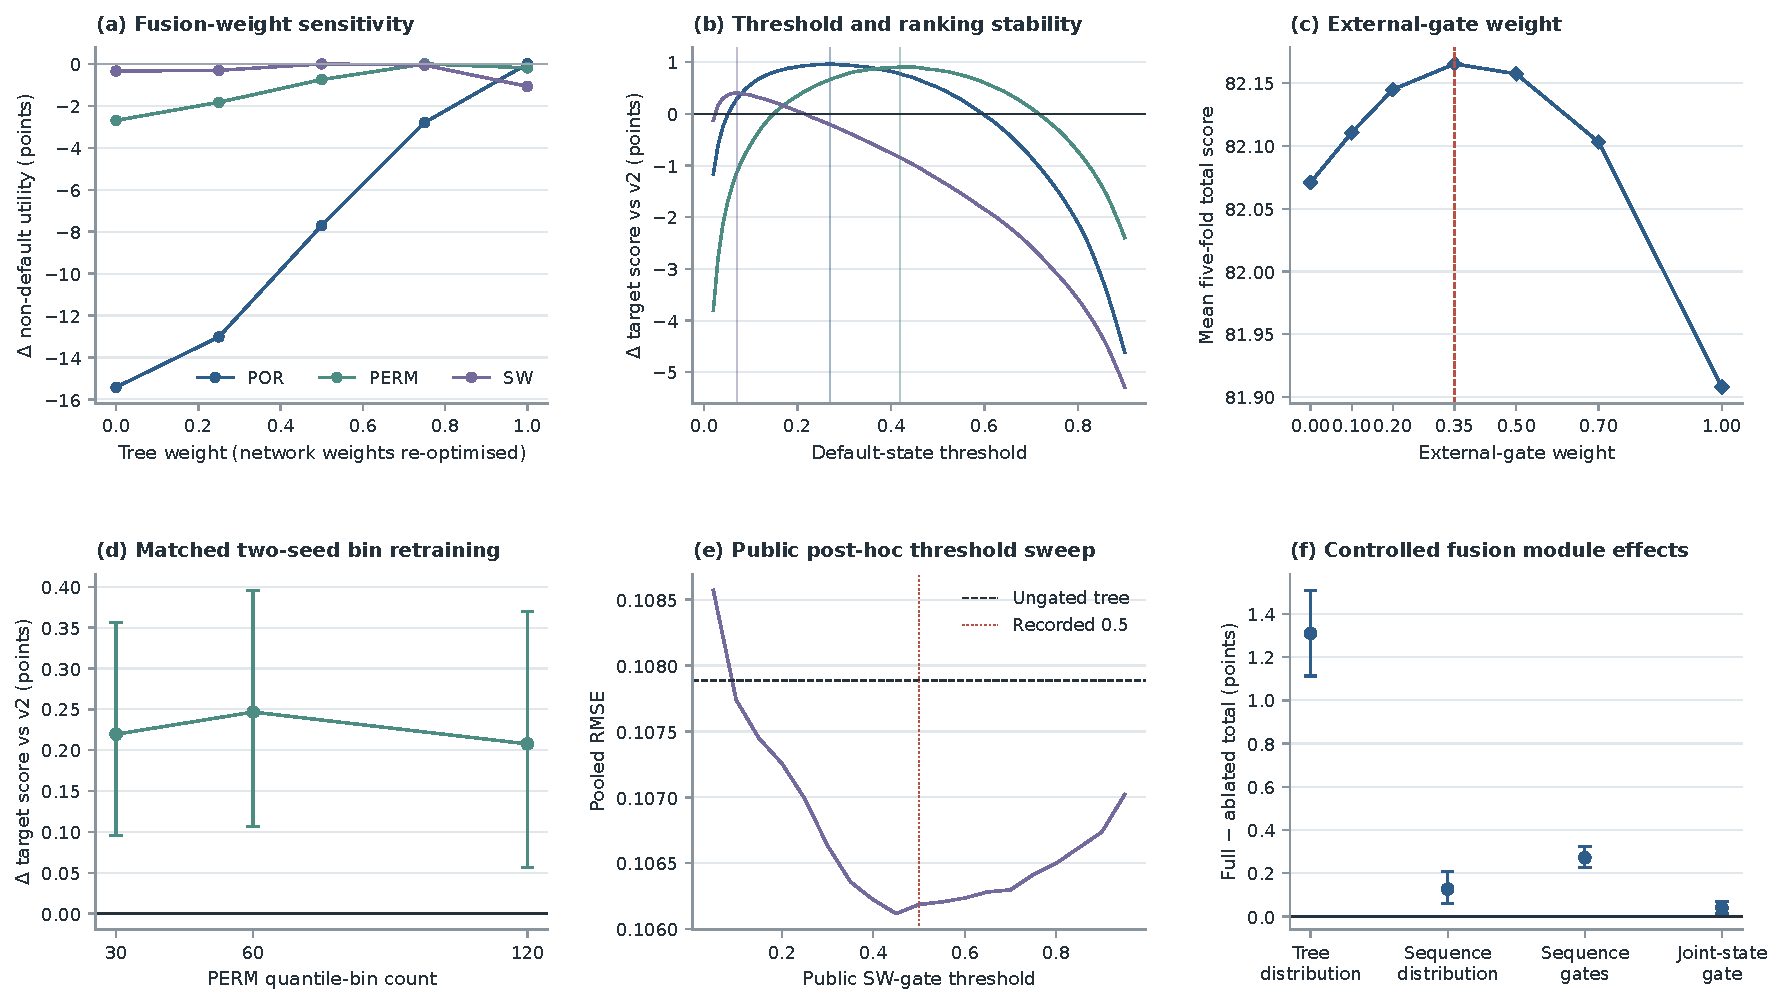
\includegraphics[width=\textwidth]{figures/reviewer_sensitivity.pdf}
\caption{系统性超参数敏感性与消融分析。(a) 连续融合权重的边际敏感性。(b) 内部决策阈值相对于 v2 基线的变化响应。(c) 冻结外部独立门控权重在各折上的遍历表现。(d) 渗透率分位数分箱数的双种子匹配重训实验。(e) 公开 Volve 测试集上的阈值敏感性遍历。(f) 留一消融实验影响值及其按井 Bootstrap 置信区间。}
\label{fig:sensitivity}
\end{figure}

将外部门控混合权重（$w_{\mathrm{ext}}$）从 0.10 遍历至 0.50，在全部五个验证折上均取得了相较于未融合预测（$w_{\mathrm{ext}} = 0$）的稳定改进。在历史推荐值 0.35 处取得了最高的平均折得分（82.165 对比纯内部门控的 82.071），而若仅采用外部门控则导致得分下滑至 81.908（图~\ref{fig:sensitivity}c）。单折的最优权重分布在 0.20 至 0.50 之间，证明适度的集成混合具有明确价值，同时也印证了工程中并不存在唯一孤立的尖锐全局最优值。

在公开 Volve 基准上，在测试的 19 个 $\mathrm{SW}$ 决策阈值中，有 18 个均显著优于未设门控的决策树（图~\ref{fig:sensitivity}e）。事后最优阈值出现在 $\tau = 0.45$ 处（RMSE 达 0.106118），相较于默认值 0.50 仅产生 0.000069 的微小差异。这一现象再次证实了合并评价指标在阈值层面的高鲁棒性，同时保留了先前观察到的井间异质性。

最后，在渗透率目标上针对 $K \in \{30, 60, 120\}$ 分位数分箱执行的匹配从头重训实验揭示了非单调的扩展规律。30、60 与 120 个分箱下的渗透率单项得分分别为 0.89662、0.89689 与 0.89650。尽管在五折中的四折（以及 $92.4\%$ 的 Bootstrap 抽样中）60 个分箱均录得最优表现，但各分箱配置之间的差异极为微小且高度收敛：$30 - 60$ 分箱的差异为 $-0.000271$（$95\%$ 置信区间 $[-0.000600, 0.000098]$），$60 - 120$ 分箱的差异为 $+0.000390$（$95\%$ 置信区间 $[0.000103, 0.000704]$）。模型性能并未随分箱分辨率的提升呈现单调增长，表明高密度离散化迅速遭遇边际效应递减。

\section{负对照与中性对照实验}
\label{sec:negative}
为了全面划定预测框架的技术边界与架构权衡，表~\ref{tab:negative} 汇总了在系统探索过程中明确记录的负对照与中性对照实验案例。具体而言，针对 $\mathrm{SW}$ 采用 60 分箱连续概率分布替代简单状态分类，单项效用仅从 0.7484 轻微变为 0.7475（成对置信区间覆盖零点），表明离散默认态分类构成了主导性的性能增益来源。同理，超密集动作网格离散化、事后 Platt 概率校准、中值平滑滤波以及固定转移概率隐马尔可夫模型（HMM）\cite{rabiner1989hmm} 均未能带来统计增益，其核心原因在于时序平滑操作往往会抹杀具有关键地质意义的薄油气层陡峭边界跳变。基于动态时间规整（DTW）的测井曲线对齐仅使复合总分产生 81.63 至 81.64 的微小涨落。在公开 Volve 基准上，门控机制在 101 井表现出轻度敏感性，且 18 阶段完整深层时序网络在所有 4 口未见测试井上均劣于基线。这些中性与负向对照有力证实：模型综合性能完全受制于特定的表征协同机制，绝非源自网络架构复杂度的盲目堆叠。

\begin{table}[t]
\centering
\caption{本研究所记录的负对照与中性对照实验系统汇总。}
\label{tab:negative}
\footnotesize
\begin{tabular}{>{\raggedright\arraybackslash}p{.28\textwidth}>{\raggedright\arraybackslash}p{.38\textwidth}>{\raggedright\arraybackslash}p{.24\textwidth}}
\toprule
所测试技术探索 & 实测经验观测 & 算法机理剖析 \\
\midrule
$\mathrm{SW}$ 60 分箱连续分布 & 效用：0.7484 $\to$ 0.7475 & 离散类别主导，连续细分无效 \\
DTW 测井曲线对齐 & 评分：81.63 $\to$ 81.64 & 曲线自相关使得非线性对齐冗余 \\
公开基准 $\mathrm{SW}$ 门控（101 井） & RMSE：0.12295 $\to$ 0.12334 & 局部井间微相存在地质非均质性 \\
Volve 上的完整 v4 时序链 & RMSE：0.14695 对比 0.10619 (树) & 小样本井网环境下发生严重过拟合 \\
\bottomrule
\end{tabular}
\end{table}

\section{讨论}
\label{sec:discussion}
本研究揭示的核心洞见在于：面向测井曲线分析的机器学习架构设计，必须精准契合底层储层岩石物理的失效模式与实际生产部署指标。梯度提升决策树能够在高维异构特征空间中提供高度稳健的单点数值回归，深层时序网络能够为沉积相带与储层流体界面判别补充关键的空间层序上下文，而指标对齐动作解码则将概率分布宽度有效转化为符合实际工程效用的最优决策。具体而言，模型架构的功能分工清晰映射到地层物理界面的空间过渡特征：时序模型专长于刻画薄渗透夹层、流体接触面及突变岩性界面，利用纵向上下文有效克服测井仪器的围岩肩效应；而表格树模型则在物性稳定的均质储层段内部主导高精度的连续数值估计。然而，严谨受控的消融实验明确警告：这些架构增益表现出高度的目标依赖性——深层时序网络对含水饱和度的界面划分大有裨益，但对孔隙度的回归增益几乎为零。

此外，实证结果对算法的跨工区迁移能力给出了严谨的边界界定。尽管按井分组交叉验证有效遏制了空间自相关泄露，但它无法代替跨沉积盆地时所面临的复杂先验分布漂移。具有极高参数容量的 18 阶段时序模型在公开 Volve 数据集上的泛化衰退，确凿印证了重参数化深度网络在稀疏钻井环境下的迁移脆弱性。

\subsection{工程应用范畴与方法论边界}
为了将上述实证发现置于严密的油气工程应用语境中，必须对本研究的适用边界予以明确界定。本预测框架从方法论归属上属于数据驱动模型，通过专业特征比值构建、物理合法边界截断以及离散非储层默认态分层建模有机融合了岩石物理先验知识，而非直接正演多相流体渗流偏微分方程（PDE）或地质沉积动力学演化过程。此外，本基准测试严格面向历史电缆测井曲线的离线钻后储层物性定量评价场景，不覆盖随钻测井（LWD）实时流式推断与地质导向反馈，亦不涉及油藏数值模拟中的历史拟合与生产动态数据回灌闭环。因此，所得经验结论明确限定于静态、回顾性的钻后储层综合评价工况。在工业现场实际落地应用中，数据驱动模型的推断输出主要用于加速并辅助资深测井专家的解释工作流，必须配套建立持续的数据分布漂移监控、不确定性区间量化机制，并持续结合实体岩心实验与试油试采动态数据进行本地校准修正。

\section{结论}
\label{sec:conclusions}
本研究系统构建并论证了一种基于测井曲线的储层物性容差感知预测评估体系。在公开 Volve 基准上，配备含水饱和度联合门控的目标专用树模型取得了 0.10619 的领先合并 RMSE，而复杂的 18 阶段时序网络在小样本下未能成功迁移（RMSE 为 0.14695）。在内部 80 口井工业基准上，分层树--时序融合将复合效用总分显著拉升至 81.63。严格受控的消融实验与系统敏感性分析确证：性能的提升本质上源于状态边界门控与高精度数值回归之间的表征互补，同时深刻揭示了单目标异质性与阈值敏感性特征。

\section*{CRediT 作者贡献声明}
\textbf{陈旻杰}：概念构思、方法设计、软件研发、实验验证、理论分析、调查研究、数据整理、论文初稿起草、论文评审与修改。\textbf{辛嘉威}：概念构思、方法设计、软件研发、实验验证、理论分析、调查研究、论文评审与修改。\textbf{吴乘风}：调查研究、数据整理、资源协调、监督指导、论文评审与修改。

\section*{利益冲突声明}
作者声明不存在已知会影响本文所汇报工作的任何相互冲突的经济利益或个人人际关系。

\section*{生成式人工智能辅助技术声明}
作者在论文撰写过程中使用生成式人工智能工具辅助进行了学术英语润色、代码复核与排版校对，并在随后对生成内容进行了全篇人工审查与严谨修订，对本文内容的真实性、学术准确性与整体学术诚信负全部责任。

\section*{数据可用性说明}
公开 Volve/PDDA 数据集可通过 SPWLA PDDA SIG 官方代码库公开获取 \cite{pddasig2021}，并遵守 Equinor Volve 许可协议 \cite{volve2018}。内部工业基准数据集受保密协议与数据合规限制，可在满足审批条件后向大赛组委会官方邮箱提出申请（\url{mailto:aicomp@petrochina.com.cn}）。主要聚合结果、公开预测真值与复现验证脚本随补充材料同步提供。

\section*{复现性说明}
本文的完整算法源代码、公开基准复现流程、敏感性分析与受控消融实验脚本已在 GitHub 开源公布：\url{https://github.com/whiteicey/welllog-reservoir-hybrid}。公开数据集的核心运行入口为 {\small\path{reproduce_public_validation.py}}（位于 {\small\path{reproducibility/public_volve/}}）。内部基准的敏感性分析与受控消融实验脚本、冻结基准配置、环境依赖记录及输出哈希值均完整归档于论文工程目录 {\small\path{experiments/reviewer_response/}}。

\section*{致谢}
作者衷心感谢 SPWLA PDDA SIG 与 Equinor 团队开源发布 Volve 数据集，感谢昆仑大模型技术挑战赛组委会提供的大规模工业实测基准。

\section*{资助信息}
本研究未获得政府、商业或非营利组织的任何专门专项研究基金资助。

\bibliographystyle{elsarticle-num}
\begingroup
\small
\setlength{\bibsep}{2.5pt}
\bibliography{refs}
\endgroup
\end{document}
